% Comparación de embedding euclidiano vs. disco de Poincaré
% Compilar con: pdflatex hyperbolic_embedding.tex
\documentclass[tikz,border=10pt]{standalone}
\usepackage{tikz}
\usetikzlibrary{calc}

\definecolor{gdlblue}{RGB}{41, 98, 168}
\definecolor{gdlred}{RGB}{191, 49, 49}
\definecolor{gdlgreen}{RGB}{30, 130, 76}
\definecolor{gdlorange}{RGB}{217, 130, 30}
\definecolor{gdlpurple}{RGB}{118, 56, 138}
\definecolor{gdlgray}{RGB}{140, 140, 140}
\definecolor{gdlyellow}{RGB}{190, 140, 10}

\begin{document}
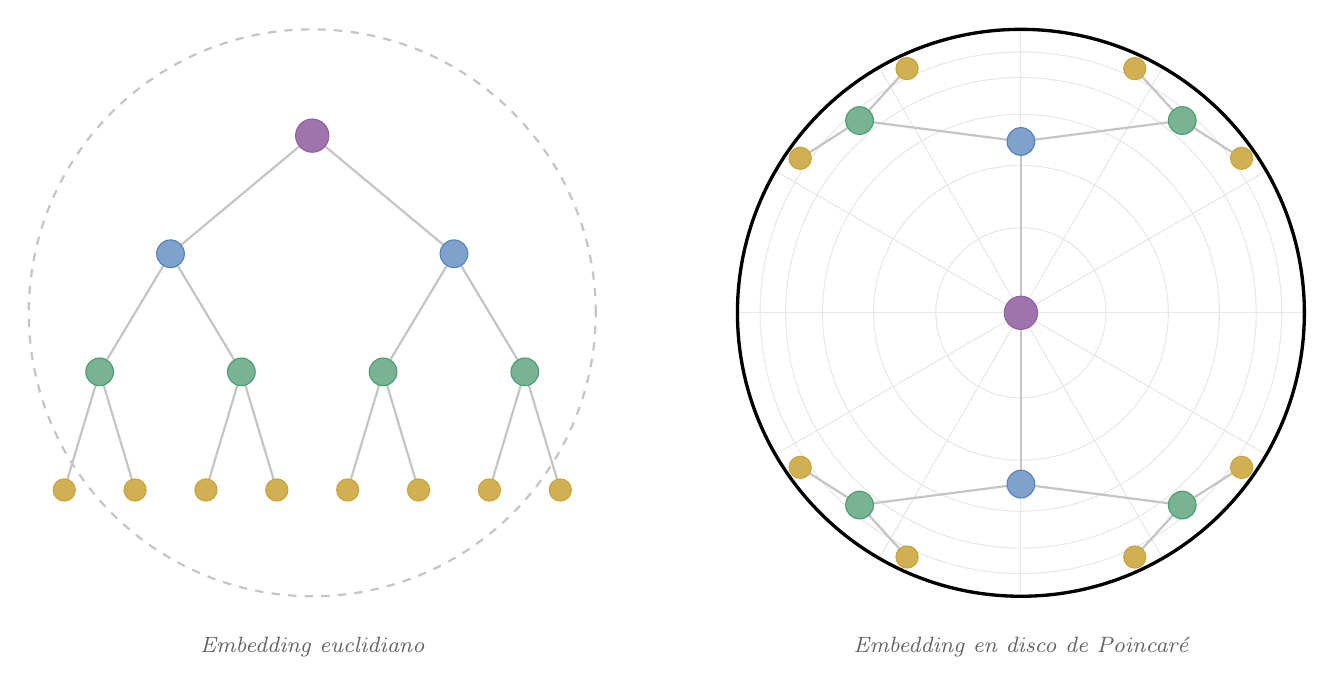
\begin{tikzpicture}[
    root node/.style={
        circle, draw=gdlpurple!80, fill=gdlpurple!70,
        minimum size=12pt, inner sep=0pt
    },
    depth1 node/.style={
        circle, draw=gdlblue!80, fill=gdlblue!60,
        minimum size=10pt, inner sep=0pt
    },
    depth2 node/.style={
        circle, draw=gdlgreen!80, fill=gdlgreen!60,
        minimum size=10pt, inner sep=0pt
    },
    leaf node/.style={
        circle, draw=gdlyellow!80, fill=gdlyellow!70,
        minimum size=8pt, inner sep=0pt
    },
    tree edge/.style={draw=gdlgray!50, line width=0.8pt},
]

% ============================================================
% LEFT PANEL: Euclidean embedding
% ============================================================
\begin{scope}[shift={(0,0)}]

    % --- Tree layout ---
    % Vertically centered: root at top, leaves at bottom
    % Total height ~4.8, centered vertically at y = -0.5
    \coordinate (r) at (0, 1.9);

    % Depth 1: 2 nodes
    \coordinate (d1-0) at (-1.8, 0.4);
    \coordinate (d1-1) at ( 1.8, 0.4);

    % Depth 2: 4 nodes
    \coordinate (d2-0) at (-2.7, -1.1);
    \coordinate (d2-1) at (-0.9, -1.1);
    \coordinate (d2-2) at ( 0.9, -1.1);
    \coordinate (d2-3) at ( 2.7, -1.1);

    % Depth 3 (leaves): 8 nodes
    \coordinate (d3-0) at (-3.15, -2.6);
    \coordinate (d3-1) at (-2.25, -2.6);
    \coordinate (d3-2) at (-1.35, -2.6);
    \coordinate (d3-3) at (-0.45, -2.6);
    \coordinate (d3-4) at ( 0.45, -2.6);
    \coordinate (d3-5) at ( 1.35, -2.6);
    \coordinate (d3-6) at ( 2.25, -2.6);
    \coordinate (d3-7) at ( 3.15, -2.6);

    % Dashed boundary circle centered on tree
    \draw[dashed, gdlgray!50, line width=0.8pt] (0,-0.35) circle (3.6);

    % Edges: root to depth 1
    \draw[tree edge] (r) -- (d1-0);
    \draw[tree edge] (r) -- (d1-1);

    % Edges: depth 1 to depth 2
    \draw[tree edge] (d1-0) -- (d2-0);
    \draw[tree edge] (d1-0) -- (d2-1);
    \draw[tree edge] (d1-1) -- (d2-2);
    \draw[tree edge] (d1-1) -- (d2-3);

    % Edges: depth 2 to depth 3
    \draw[tree edge] (d2-0) -- (d3-0);
    \draw[tree edge] (d2-0) -- (d3-1);
    \draw[tree edge] (d2-1) -- (d3-2);
    \draw[tree edge] (d2-1) -- (d3-3);
    \draw[tree edge] (d2-2) -- (d3-4);
    \draw[tree edge] (d2-2) -- (d3-5);
    \draw[tree edge] (d2-3) -- (d3-6);
    \draw[tree edge] (d2-3) -- (d3-7);

    % Draw nodes on top of edges
    \node[root node] at (r) {};
    \node[depth1 node] at (d1-0) {};
    \node[depth1 node] at (d1-1) {};
    \foreach \i in {0,...,3} {
        \node[depth2 node] at (d2-\i) {};
    }
    \foreach \i in {0,...,7} {
        \node[leaf node] at (d3-\i) {};
    }

    % Label (aligned with right panel)
    \node[font=\footnotesize\itshape, text=gdlgray!70!black] at (0, -4.6)
        {Embedding euclidiano};
\end{scope}

% ============================================================
% RIGHT PANEL: Poincaré disk embedding
% ============================================================
\begin{scope}[shift={(9.0, -0.35)}]

    % Disk radius (same visual size as left panel circle)
    \pgfmathsetmacro{\R}{3.6}

    % --- Tessellation (subtle background) ---
    % Concentric circles at hyperbolic-spaced radii
    \foreach \rad in {0.30, 0.52, 0.70, 0.83, 0.92} {
        \draw[gdlgray!20, thin] (0,0) circle (\rad*\R);
    }
    % Radial lines (12 lines, every 30 degrees)
    \foreach \ang in {0, 30, 60, 90, 120, 150, 180, 210, 240, 270, 300, 330} {
        \draw[gdlgray!20, thin] (0,0) -- ({\ang}:\R);
    }

    % Unit disk boundary
    \draw[black, line width=1.2pt] (0,0) circle (\R);

    % --- Hyperbolic tree layout ---
    % tanh mapping: r = tanh(depth * 0.7) * R
    % tanh(0.7) = 0.6044  -> level 1 radius
    % tanh(1.4) = 0.8854  -> level 2 radius
    % tanh(2.1) = 0.9705  -> level 3 radius (well inside boundary)
    \pgfmathsetmacro{\rone}{0.6044*\R}   % ~2.176
    \pgfmathsetmacro{\rtwo}{0.8854*\R}   % ~3.187
    \pgfmathsetmacro{\rthree}{0.9505*\R} % ~3.422 (slightly reduced to avoid touching boundary)

    % Root at center
    \coordinate (pr) at (0, 0);

    % Depth 1: 2 nodes, angles 90 and 270
    \coordinate (pd1-0) at ({90}:{\rone});
    \coordinate (pd1-1) at ({270}:{\rone});

    % Depth 2: 4 nodes
    % Children of pd1-0 (at 90deg): spread to 50, 130
    % Children of pd1-1 (at 270deg): spread to 230, 310
    \coordinate (pd2-0) at ({50}:{\rtwo});
    \coordinate (pd2-1) at ({130}:{\rtwo});
    \coordinate (pd2-2) at ({230}:{\rtwo});
    \coordinate (pd2-3) at ({310}:{\rtwo});

    % Depth 3: 8 leaves
    % Children of pd2-0 (at 50): 35, 65
    % Children of pd2-1 (at 130): 115, 145
    % Children of pd2-2 (at 230): 215, 245
    % Children of pd2-3 (at 310): 295, 325
    \coordinate (pd3-0) at ({35}:{\rthree});
    \coordinate (pd3-1) at ({65}:{\rthree});
    \coordinate (pd3-2) at ({115}:{\rthree});
    \coordinate (pd3-3) at ({145}:{\rthree});
    \coordinate (pd3-4) at ({215}:{\rthree});
    \coordinate (pd3-5) at ({245}:{\rthree});
    \coordinate (pd3-6) at ({295}:{\rthree});
    \coordinate (pd3-7) at ({325}:{\rthree});

    % Edges: root to depth 1
    \draw[tree edge] (pr) -- (pd1-0);
    \draw[tree edge] (pr) -- (pd1-1);

    % Edges: depth 1 to depth 2
    \draw[tree edge] (pd1-0) -- (pd2-0);
    \draw[tree edge] (pd1-0) -- (pd2-1);
    \draw[tree edge] (pd1-1) -- (pd2-2);
    \draw[tree edge] (pd1-1) -- (pd2-3);

    % Edges: depth 2 to depth 3
    \draw[tree edge] (pd2-0) -- (pd3-0);
    \draw[tree edge] (pd2-0) -- (pd3-1);
    \draw[tree edge] (pd2-1) -- (pd3-2);
    \draw[tree edge] (pd2-1) -- (pd3-3);
    \draw[tree edge] (pd2-2) -- (pd3-4);
    \draw[tree edge] (pd2-2) -- (pd3-5);
    \draw[tree edge] (pd2-3) -- (pd3-6);
    \draw[tree edge] (pd2-3) -- (pd3-7);

    % Draw nodes on top of edges
    \node[root node] at (pr) {};
    \node[depth1 node] at (pd1-0) {};
    \node[depth1 node] at (pd1-1) {};
    \foreach \i in {0,...,3} {
        \node[depth2 node] at (pd2-\i) {};
    }
    \foreach \i in {0,...,7} {
        \node[leaf node] at (pd3-\i) {};
    }

    % Label (vertically aligned with left panel)
    \node[font=\footnotesize\itshape, text=gdlgray!70!black] at (0, -4.25)
        {Embedding en disco de Poincar\'{e}};
\end{scope}

\end{tikzpicture}
\end{document}
